\chapter{Introduction} \label{chap:Introduction}

\section{Zoonoses and the risks of pandemics}

In times where infectious disease outbreaks become more frequent and sometimes even reach global appearance, unpredictable effects on humans, wildlife and whole ecosystems are inevitable \autocite{schmeller_biodiversity_2020}. Growing human population and persisting poverty has harmful impact on the biodiversity and results in degradation of natural habitats and more frequent human-wildlife contacts  \autocite{schmeller_biodiversity_2020}. Therefore, increasing numbers of zoonoses, transfers of animal pathogens on humans, arise and are a major driving force in pathogen emergence on humans in recent decades \autocite{jones_global_2008}. Most of the human pathogens emerging lately are of animal origin, indeed, up to 75\% \autocite{woolhouse_risk_2001}. Well-known examples of zoonoses are avian and swine flu \gls{HIV}, ebola, \gls{MERS} and \gls{SARS} including the current circulating COVID-19 \autocite{van_reeth_avian_2007, sharp_origins_2011, suwantarat_risks_2015, verity_estimates_2020}.

\vspace{1em}

While zoonoses can be of viral, bacterial and parasitic nature, emergences of higher magnitude, like the mentioned well-known examples, are often linked back to viral infections \autocite{woolhouse_risk_2001}. Harmfulness of viral infections can be diverse, ranging from mostly no sign of infection in the natural hosts to very severe symptoms or death in accidental hosts \autocite{wahlgren_influenza_2011}. In contrast to natural hosts, humans, accidental hosts to, e.~g.~, the West Nile Virus, develop disease patterns upon infection and, thereby, are not able to support the virus life cycle \autocite{gea-banacloche_west_2004}. High variety in host circulation and transmission ways from such natural or intermediate onto humans as accidental hosts, with long infectious periods without symptoms and high transmission pace have a high risk of pandemic events \autocite{jamison_chapter_2017}. A prominent virus detected in a variety of hosts and known for reoccurring local and global outbreaks in the past is \gls{IAV}, member of the \textit{Orthomyxoviridae} family and also commonly known as flu \autocite{wahlgren_influenza_2011}. Analysis indicate a 1\% chance of a pandemic with millions of deaths every year and is, therefore, the pathogen most likely to be responsible for a sudden severe pandemic \autocite{jamison_chapter_2017}. 

\section{Life-cycle and structure of the \textit{Influenza A Virus}}

\begin{figure}
    \centering
    %\begin{adjustbox}{minipage=\dimexpr\textwidth-2\fboxsep-2\fboxrule,fbox}
    \begin{subfigure}[b]{0.475\textwidth}
        \caption[\textit{Alphainfluenzavirus}]{\textbf{\textit{Alphainfluenzavirus}}}
        \label{subfig:Influenza_A}
        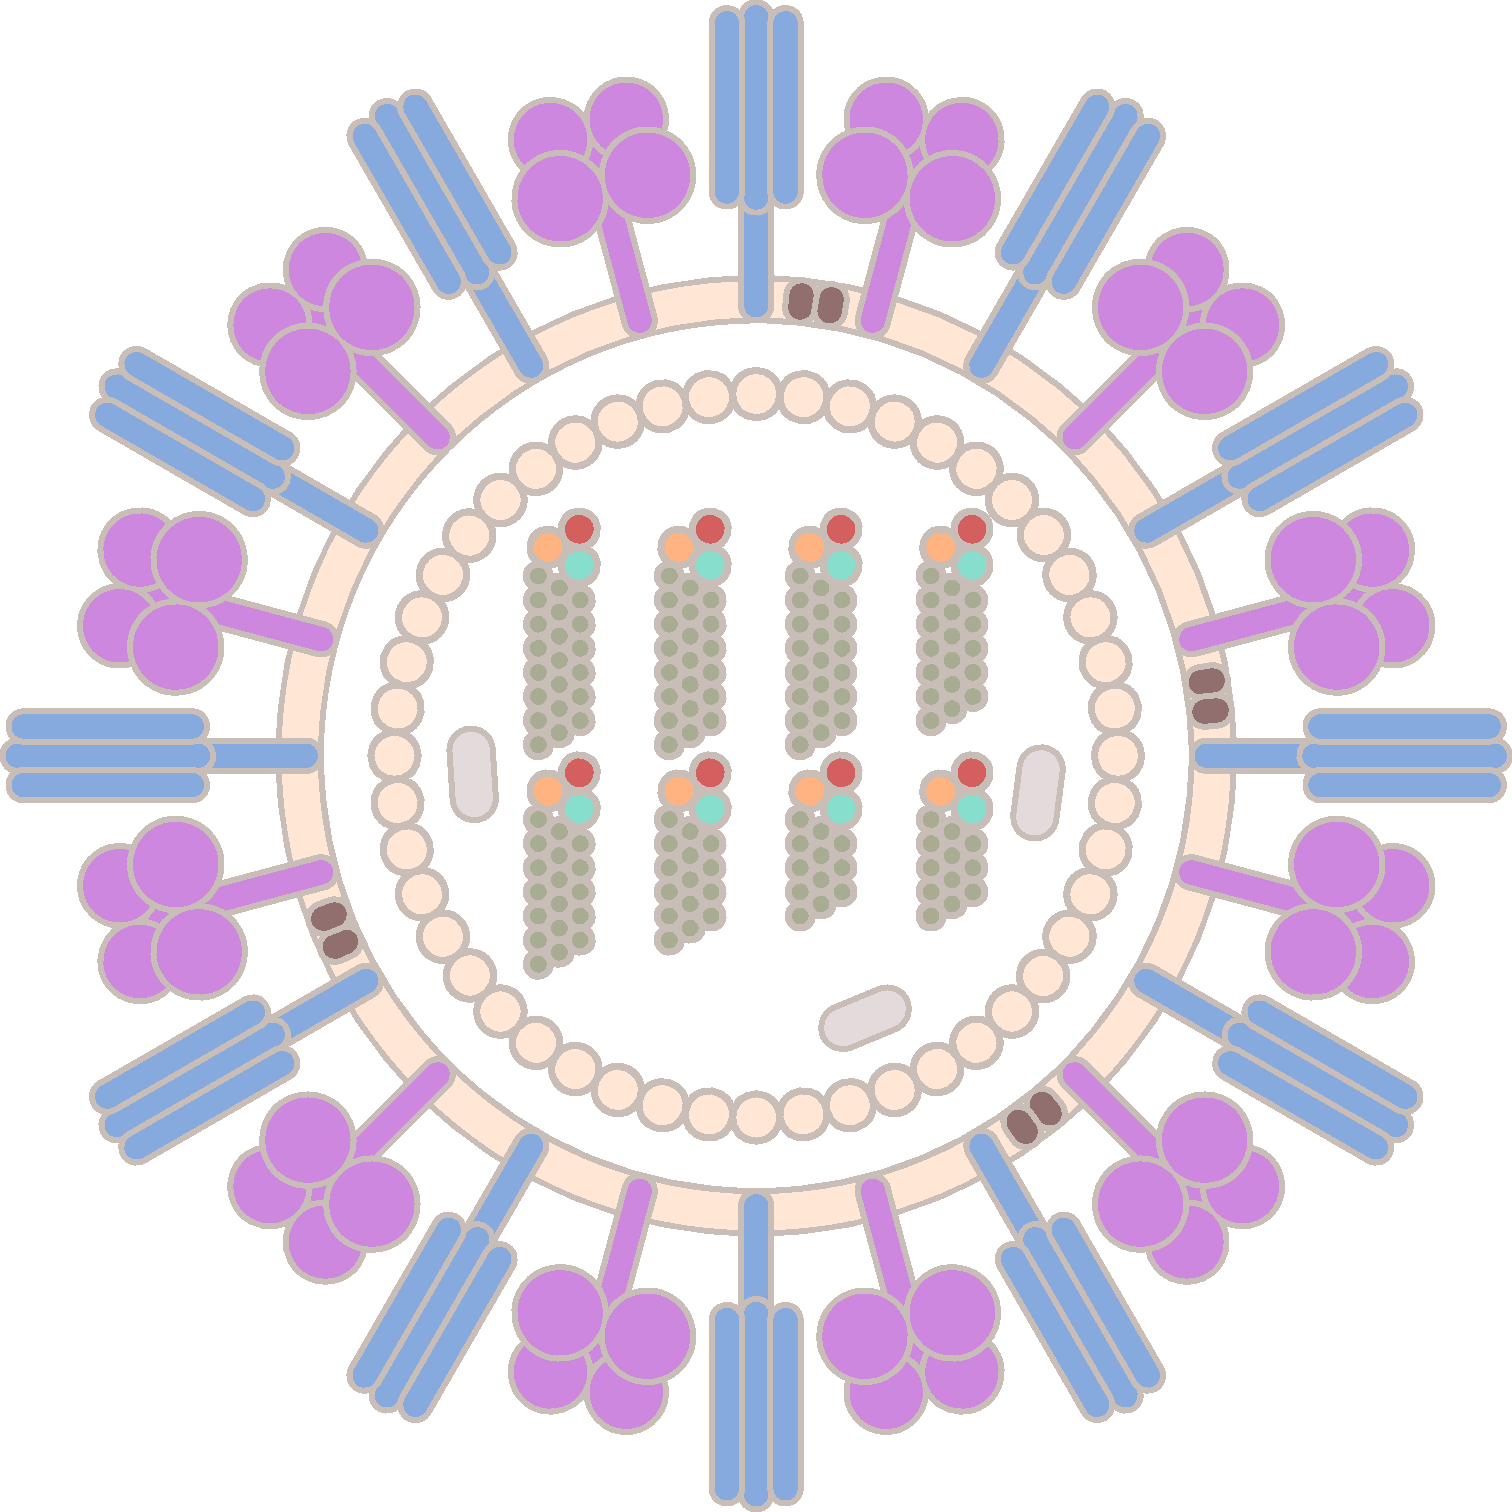
\includegraphics[width=\textwidth]{Graphics/Influenza_A.pdf}
    \end{subfigure}
    \hfill
    \begin{subfigure}[b]{0.475\textwidth}
        \caption[\textit{Betainfluenzavirus}]{\textbf{\textit{Betainfluenzavirus}}}
        \label{subfig:Influenza_B}
        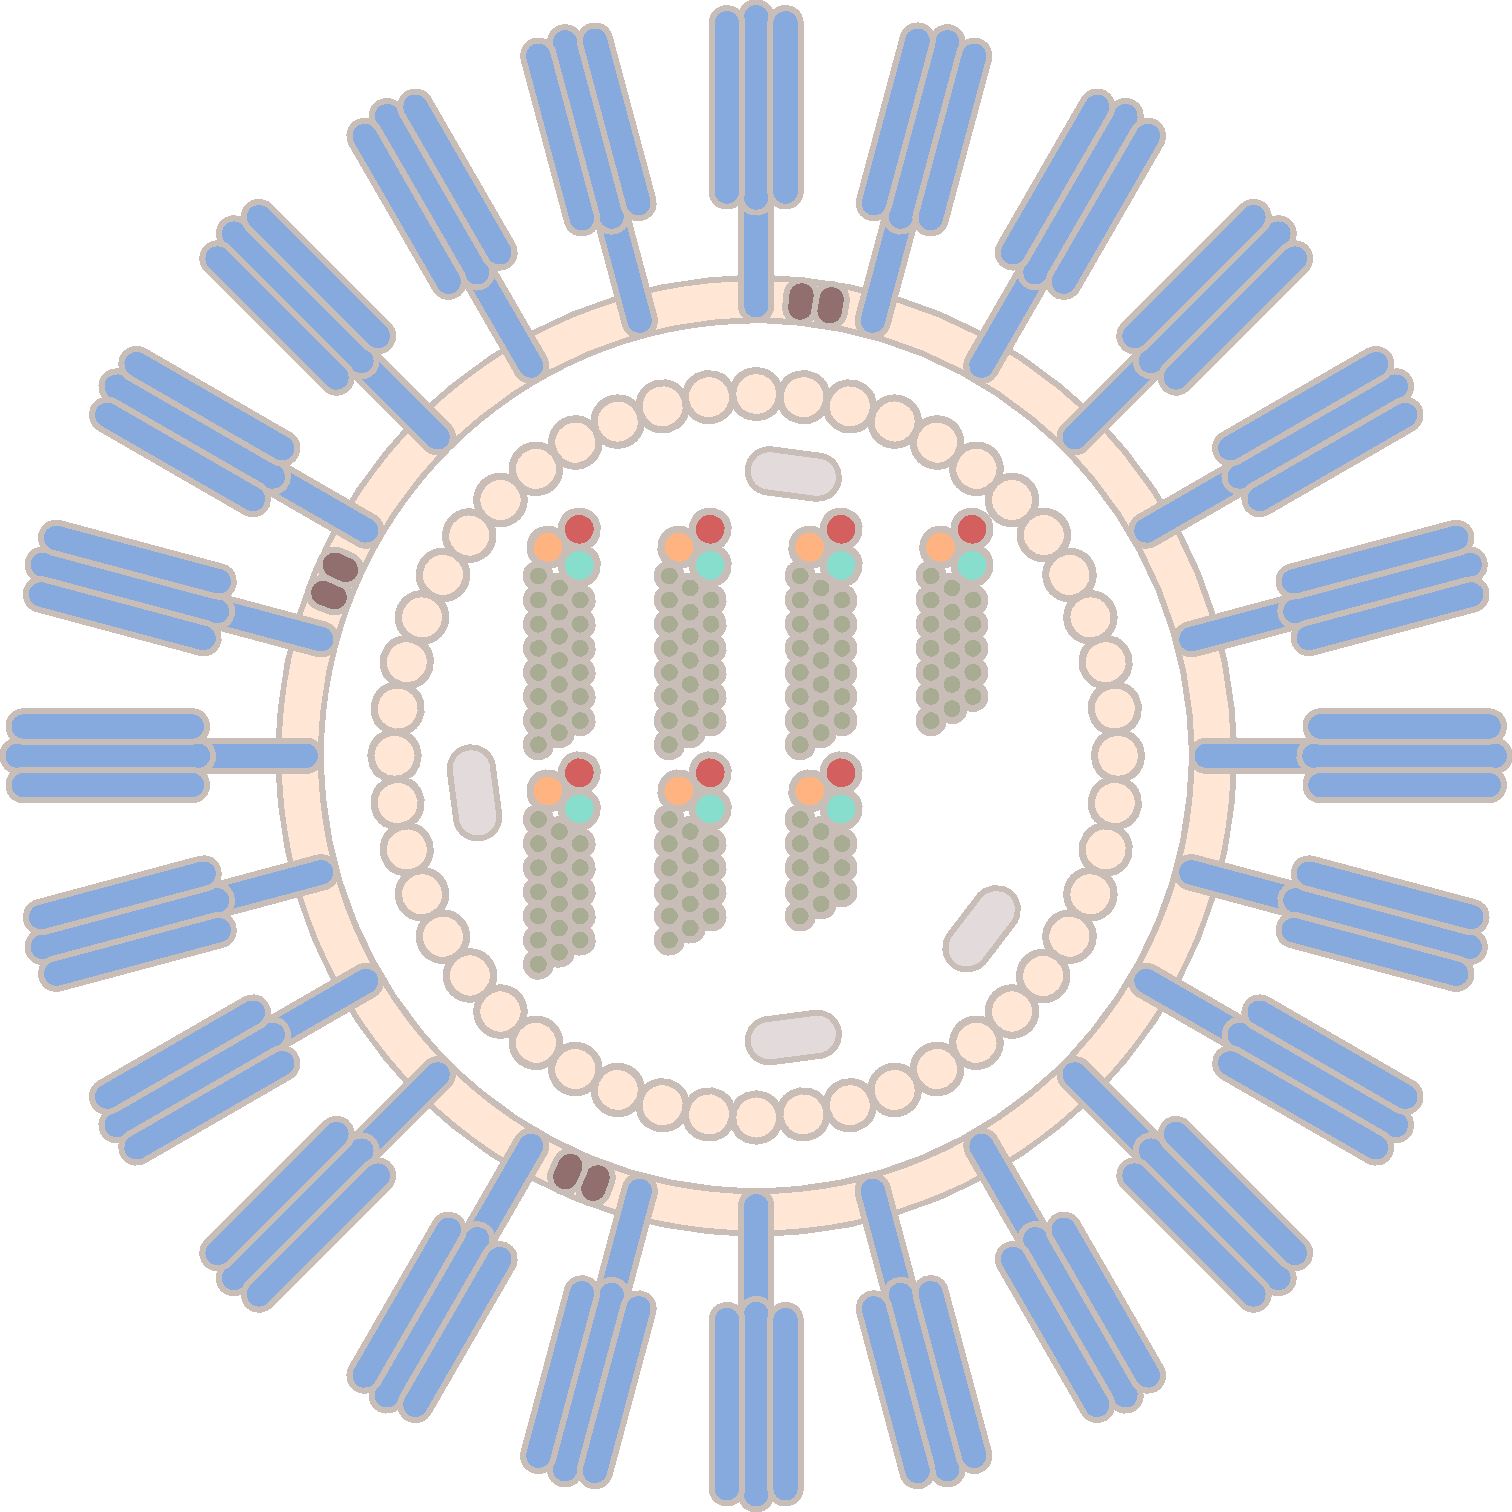
\includegraphics[width=\textwidth]{Graphics/Influenza_B.pdf}
    \end{subfigure}
    %\end{adjustbox}
    \caption[\textit{Orthomyxoviridae}]{\textbf{\textit{Orthomyxoviridae}.} .}
    \label{fig:Orthomyxoviridae}
\end{figure}

In humans, infection by \gls{IAV} affects the upper respiratory tract \autocite{julkunen_inflammatory_2000}. General symptoms like fever, cough and headache characterize the infection \autocite{julkunen_inflammatory_2000}. In some cases complications can occur, resulting in primary viral pneumonia or secondary bacterial pneumonia by bacterial infection \autocite{julkunen_inflammatory_2000}. The virus particles of \gls{IAV}, called virions, are spherical in shape, 80–120nm in size and enveloped by the hosts cell membrane lipids \autocite{oxford_chapter_1987, mudhakir_learning_2009, cann_chapter_2016}. These virions can sustain extensive forces in the hosts body and even survive deformation to around 33\% of the its total diameter \autocite{schaap_effect_2012}. Epithelial cells in the tissue of the respiratory tract, are the main infection area of the virions \autocite{oxford_chapter_1987}. The \gls{IAV} virions attach themselves to the host cells with their surface glycoproteins, the tetrameric \gls{NA} and the trimeric \gls{HA} and enter the cells by clathrin-mediated endocytosis (\autoref{subfig:Influenza_A}) \autocite{wilson_structure_1981, varghese_structure_1983, jones_global_2008, mudhakir_learning_2009}. Equilibration of pH in the process of endocytosis involve the transmembrane protein \gls{M2} of \gls{IAV} \autocite{pielak_influenza_2011}. The surface glycoprotein tails are also connected to the second layer in the \gls{IAV} virions, the \gls{M1} \autocite{ali_influenza_2000}. Following the endocytosis the \gls{RNP} complexes are carried to the hosts cells nucleus by \gls{NPC} for virus replication \autocite{eisfeld_at_2015}. These \gls{RNP} complexes contain the viral \gls{ssRNA}, holding the genetic information, bound to multiple \glspl{NP} and the polymerase complex \autocite{eisfeld_at_2015}. The trimeric polymerase complex including the \gls{PB1}, \gls{PB2} and \gls{PA} is essential for viral replication in the hosts nucleus \autocite{area_3d_2004, eisfeld_at_2015}. \gls{IAV} is a segmented virus, one virion of \gls{IAV} contains eight different short \glspl{ssRNA}, called segments, encoding in total 14 viral proteins \autocite{eisfeld_at_2015}. In the nucleus the eight \glspl{ssRNA} are replicated and transcribed to \glspl{mRNA} with the latter translated to the virions proteins in the cytoplasm \autocite{eisfeld_at_2015}. The translated \gls{NEP}, \gls{M1}, \gls{NP} and proteins of the polymerase complex are imported by the \gls{NPC} to build new \glspl{RNP} with the replicated genomes and enable the nuclear exit \autocite{eisfeld_at_2015}. By budding through the plasma membrane with the translated \gls{M2}, while incorporating the translated \gls{HA} and \gls{NA} into the surface, new virions are released \autocite{eisfeld_at_2015}.

\section{Evolution of the \textit{Influenza A Virus}}

Present day research, indicate mallards \textit{(Anas platyrhynchos)} as main reservoir and natural host of \glspl{LPAIV} \autocite{jourdain_influenza_2010}. Studies on Pekin ducks, descended from mallards, have shown minor immune responses and antibody production to the infection with \gls{IAV} strains and the possibility of a reinfection after two months with the same strain \autocite{kida_duck_1980}. Strains are lines of \gls{IAV} related to a specific location and time point \autocite{cann_chapter_2016}. Less dangerous strains of \gls{IAV}, called \glspl{LPAIV}, seem to repeatedly circulate in duck species and may evolve into human pathogenic strains by zoonoses \autocite{jourdain_influenza_2010}. Simple transmission over species is not enough to start a pandemic though, therefore, better understanding of the mostly unknown genetic changes vital for zoonotic events is required \autocite{van_reeth_avian_2007}. Circulation of these strains in aquatic bird species with continued evolution enable the transmission possibilities to humans, lower animals, and other birds \autocite{webster_chapter_1999}. The evolution occurs in all segments of the \gls{IAV} but is most prominent in \gls{HA} and \gls{NA} \autocite{webster_chapter_1999}. Infection is mostly dependent on these surface glycoproteins, building the serotype, of the virus, as they are crucial for attachment to host cells \autocite{cann_chapter_2016}. Significant variation in the surface glycoproteins mostly occur by reassortment, also called genetic shift and point mutations, also called antigenic drift \autocite{webster_chapter_1999}. Current classifiaction of \gls{IAV} by the subtypes naming convention is solely based on the surface proteins as proposed in \textcite{noauthor_revision_1980}. In the publication the previous subtypes proposed in \textcite{noauthor_revised_1971} consisting of H0 to H3, Hsw1, Heq1, Heq2 and Hav1 to Hav10 were replaced by the known subtypes H1 to H12 for \gls{HA} and in a similar similar for \gls{NA} by replacement of N1, N2, Neq1, Neq2 and Nav1 to Nav6 in favor of N1 to N9. The subtype convention was changed due to characterization of the RNA based on immunological relationships as described in \textcite{noauthor_reconsideration_1979} prior to the final subtype change. The subtypes were also grouped according to the sequence homology of the \gls{NS1} protein with some major differences \autocite{noauthor_reconsideration_1979}. Still, due to missing \gls{NS1} protein serological data only \gls{HA} and \gls{NA} were used for the classification. Other segments were not considered due to being highly conserve \autocite{noauthor_reconsideration_1979}. However, future classification involving all the segments was not negated, if appropriate \autocite{noauthor_reconsideration_1979}. Subtype convention on the surface proteins was, therefore, agreed due to not being highly conserved because of high evolutionary pressure.

\vspace{1em}

Point mutations in the segmented genome are very frequent, as the mutation rate in all RNA viruses is very high \autocite{duffy_why_2018}. Present \textit{poliovirus} research, indicate higher selection for faster replication and, therefore, acceptance of replication errors in favor of faster viral polymerases \autocite{pfeiffer_increased_2005, duffy_why_2018}. This finding is in line with research indicating the short length or segmentation of RNA viruses and the high mutation rates as evolutionary trade-off \autocite{belshaw_pacing_2008, vignuzzi_closing_2012}. Thereby, creating a cloud of offsprings, called quasispecies, with 1-2 mutations in the genome each \autocite{belshaw_pacing_2008, vignuzzi_closing_2012}. The point mutations affect the offsprings surface proteins \gls{AA} composition in the translation process, by possible missense and nonsense errors or frameshifts \autocite{parker_errors_1989, webster_chapter_1999}. Reassortment is a more drastical change in the surface proteins and likely to be related to the pasts most horrible \gls{IAV} pandemic, the spanish flu in 1918 \autocite{nelson_multiple_2008}. For reassortment induced zoonoses, there has to be a intermediate host or \glqq mixing vessel\grqq{}, most likely pigs, able to be infected by \glspl{IAV} of different hosts \autocite{shu_evidence_1994}. The hosts cells can then be co-infected by two different \glspl{IAV} and create offsprings with mixed segments \autocite{compans_influenza_2014}. All segments can be exchanged, but, in case of surface proteins of different hosts, \glspl{IAV} can occur that are able to do interspecies transmission \autocite{shu_evidence_1994}. Avian \gls{IAV} strains can, thereby, evolve to human strains by co-infection of a pig with human transferable and avian originating \gls{IAV} strains \autocite{shu_evidence_1994}. 

\section{Vaccines design and the link to reassortment}

Reassortment events are a major source of danger, since no real cure to \gls{IAV} infection is available and generation of vaccines is straining and not always as effective as expected \autocite{wahlgren_influenza_2011, wong_traditional_2013}. Furthermore, the efficacy of vaccines vary in specific populations and there are limitations to the manufacturing and the time frame of the production \autocite{wong_traditional_2013}. The strains most likely to circulate for the season are selected twice a year by the \gls{WHO}, to be included in vaccines prepared for the winters in both hemispheres \autocite{barr_epidemiological_2010}. The seasonal used \gls{IAV} vaccines target the highly mutable head domain of \gls{HA} surface proteins to stimulate immune response \autocite{wong_traditional_2013, wei_next-generation_2020}. Therefore, the \gls{IAV} vaccines efficiency vary depending on the similarity of the \gls{HA} head domain of the strains used for the vaccines and the ones circulating in the season \autocite{wei_next-generation_2020}. The accuracy of the recommendation by the \gls{WHO} is, therefore, especially crucial for the survival of humans with pre-existing conditions or humans of old age that are more prone to infection. To manufacture the vaccines, reassortment of the selected strain with a master strain is induced in eggs \autocite{wong_traditional_2013}. The resulting hybrid strain contains the selected strains surface proteins and the master strains high-growth properties necessary for production of the vaccine in the short time frame \autocite{wong_traditional_2013}. Therefore enlarging the knowledge of \gls{IAV} reassortment is important for the prediction of future pandemic strains, creation of vaccines by high-growth hybrid strains and the overall efficiency of the vaccines against circulating variable strains most likely to undergo reassortment \autocite{wong_traditional_2013, dadonaite_structure_2019}. For better understanding of \glspl{IAV} reassortment and estimation of resulting risks, the interaction mechanisms of the genome segments have to be fully discovered \autocite{dadonaite_structure_2019}. 

\section{Importance of Secondary Structure Prediction}

The eight \gls{IAV} \gls{ssRNA} segments are single-stranded chains of nucleotides, by inter- and intra-molecular base-pairing various complex arrangements with different stabilities can be build \autocite{higgs_rna_2000, dadonaite_structure_2019}. Single-stranded RNA viruses can use secondary structures on the \gls{ssRNA} as well as on the transcribed positive \gls{mRNA} for different mechanisms, like the initiation of the translation on the \gls{mRNA} by the \gls{IRES} or inter-molecular binding of different \gls{ssRNA} segments to each other \autocite{kieft_viral_2008, moss_identification_2011, dadonaite_structure_2019}. \textcite{gerber_selective_2014} described the selective \glspl{IAV} packaging by segment interactions with consequences for reassortment. It is assumed, that different interactions favor reassortment while others prevent specific segment incorporation in the reassortant virus. Fully understanding the conserved structures and interactions of \glspl{IAV} segments would, thereby, enlarge our knowledge of \gls{IAV} to a great extend. Prediction of these viral secondary structures is mostly done by lab methods \textit{in virio} and \textit{in vitro} or computationally with \textit{in silico} methods, with the latter mostly based on thermodynamic calculations alone \autocite{moss_identification_2011, dadonaite_structure_2019}. \textit{In virio} methods involve modification inside a virion and \textit{in vitro} methods involve modification on transcribed RNA in a probe, both can used with SHAPE-MaP and SPLASH methods \autocite{smola_selective_2015, dadonaite_structure_2019}. Following the lab methods structure prediction is performed by tools using the insight of the lab methods for better accuracy, in \textcite{dadonaite_structure_2019} using \texttt{IntaRNA} \autocite{}. Prediction of present day secondary structures on single sequences by \textit{in silico} thermodynamic energy minimization calculations can be performed \texttt{RNAfold} \autocite{}. Both lab methods can only be used to analyze secondary structure folding on single viruses at once, but reveal structures at single-nucleotide resolution \autocite{dadonaite_structure_2019}. \textit{In silico} methods that are used without support by experiments are not limited by prediction on single viruses, only require prior sequenced genomes \autocite{moss_identification_2011, dadonaite_structure_2019}. Since \textit{in silico} methods can be used on a higher number of sequences at once, consensus structures can be predicted together to find conserved, possibly equal folding regions in the sequenced genomes by prior multiple sequence alignments \autocite{moss_identification_2011}. 

\section{Alignments and Clustering}

Aligning multiple sequences to each other is possible by a number of different methods nowadays. The core of most multiple alignment methods were created by \textcite{needleman_general_1970} with an algorithm usable to aligns two sequences in a pairwise manner using fast dynamic programming. The algorithm was intended to be used solely on proteins but could be transfered to any problems involving pairwise distance and was soon used for nucleotide sequence comparisons \autocite{phillips_multiple_2000}. Other algorithms were created in the following years but the one proposed by Needleman and Wunsch was soon used to not only align two sequences but multiple sequences creating the possibility sequence comparisons of multiple sequences \autocite{phillips_multiple_2000}. Due to inability to be used on high numbers of sequences other algorithms, like the one proposed by \textcite{feng_progressive_1987}, were created that did not offer the same accuracy but could be performed on higher number of sequences, thereby, creating first heuristic multiple sequence alignment methods. The way for present multiple sequence alignments was paved, offering the possibility to align higher numbers of sequences in reasonable time. Present day multiple alignment tools offering global comparisons of the complete sequences are still based on these heuristic methods. Famous ones are up-to-date versions of \texttt{CLUSTALW} first proposed in \textcite{thompson_clustal_1994} and \texttt{T-COFFEE} proposed in \textcite{notredame_t-coffee_2000}. While steps in terms of accuracy had been made in the development of newer versions, calculations still have high CPU times and hardware offering high amounts of computational power are still needed \autocite{katoh_mafft_2002}. Other alignment methods exist searching for similar short profiles in the sequences and extend these matches. \texttt{MAFFT} first proposed in \textcite{katoh_mafft_2002} and evolved to the present day version as described in \textcite{katoh_mafft_2013} uses \gls{FFT} for similar profile search, resulting in faster and less costly nucleotide sequence comparison. \texttt{MUSCLE} also prominent for \glspl{MSA} creation is based on k-mers profiles instead, also improving speed \autocite{edgar_muscle_2004}. Higher numbers of aligned in shorter time-spans enable searching for conserved structures in a higher magnitude. \glspl{MSA} created by the available present day tools can be used in structure predictions by e.~g.~, \texttt{RNAalifold} \autocite{bernhart_rnaalifold_2008}.

\vspace{1em}

Since \textit{in silico} methods are based on sole predictions involving thermodynamic calculations, the choice of a set to use when aiming to make statements about higher amounts of sequences is crucial. Prediction of conserved consensus structures is, therefore, highly fragile in terms of high genomic differences of the used sequences. Prior clustering to discover related groups can be helpful in improving the accuracy of consensus structures as performed in \textcite{moss_identification_2011} for prediction of a tetraloop structure. Clustering techniques are broadly used to discover new insights of biological data, not only to predict more accurate structures in \gls{IAV} segments, but also to be used on post-genomic data in all fields of bioinformatics knowledge\autocite{handl_computational_2005}. Clustering methods exist based on entirely different concepts to separate the data. They can split given data in groups by connectedness, compactness or spatial separation of data points \autocite{handl_computational_2005}. By separation based on compactness, the method aims to reduce the intra-cluster variation as much as possible, thereby, mostly creating spherical clusters (\autoref{subfig:Connectedness}) \autocite{handl_computational_2005}. The concept of connectedness connects neighbors to each other, thus, creating chains of associated data points (\autoref{subfig:Connectedness}). The clusters are mostly arbitrarily shaped. Spatial separation is a concept aiming for splitting the data in different regions and is related to the concept of connectedness \autocite{handl_computational_2005}. Existing clustering algorithms try to best separate the data based on these concepts. Still, no existing clustering algorithm can take all of these concepts into consideration. Most clustering algorithms follow the principle of either connectedness including spatial separation, like hierarchical clustering algorithms, or the compactness concept, like density-based clustering algorithms \autocite{handl_computational_2005}. Hierarchical clustering algorithms can be used by starting with each datapoint in a single cluster and merging while climbing the hierachy, called agglomerative or divisive, when starting in on cluster and dividing in smaller ones. Prominent widely used examples for agglomerative hierarchical clustering are the \gls{UPGMA} method, that is also present in \texttt{MAFFT} for guide tree creation or the recent published \texttt{HDBCSCAN} tool \autocite{katoh_mafft_2002, mcinnes_hdbscan_2017}. A well-known examples for density-based clustering is the tool \texttt{DBSCAN} \autocite{madhulatha_overview_2012, schubert_dbscan_2017}. Regardless of which clustering methods is used, there is always a threshold that has to be defined in order for the algorithm to work as expected (\autoref{subfig:Connectedness}). Visual inspection on the clustering is not always possible making these threshold parameters a tough choice. Hierarchical clustering methods need a threshold to define the cutoff in the tree and density-based methods depend on choosing the size of an area with a given density to be handled as cluster. Estimation of a reasoned number of clusters is possible in hierarchical clustering methods by the elbow method, thus, reverse estimating the threshold parameter necessary for the number of clusters \autocite{madhulatha_overview_2012}. Clustering methods, like \texttt{USEARCH} and \texttt{CD-HIT}, that are especially developed to be used for sequence clustering, require a threshold based on sequence similarity only. However, the majority of cluster tool use data points as vectors for clustering. The dimensionality of these vectors is dependent on the amount of information. Using vectors with a high amount of information for clustering requires lowering the dimensionality of the data prior to clustering. Therefore, combination of the clustering with methods, that reduce dimensionality is crucial in the most cases. Widely used methods for reducing the dimensionality of vectors are \texttt{PCA}, \texttt{t-SNE} and \texttt{UMAP}. Choosing the right amount of preserved information in combination with wisely selected thresholds define, thus, a well conducted high-dimensional vector clustering. 

\begin{figure}
    \centering
    %\begin{adjustbox}{minipage=\dimexpr\textwidth-2\fboxsep-2\fboxrule,fbox}
    \begin{subfigure}[b]{0.475\textwidth}
        \caption[Compactness]{\textbf{Compactness}}
        \label{subfig:Compactness}            
        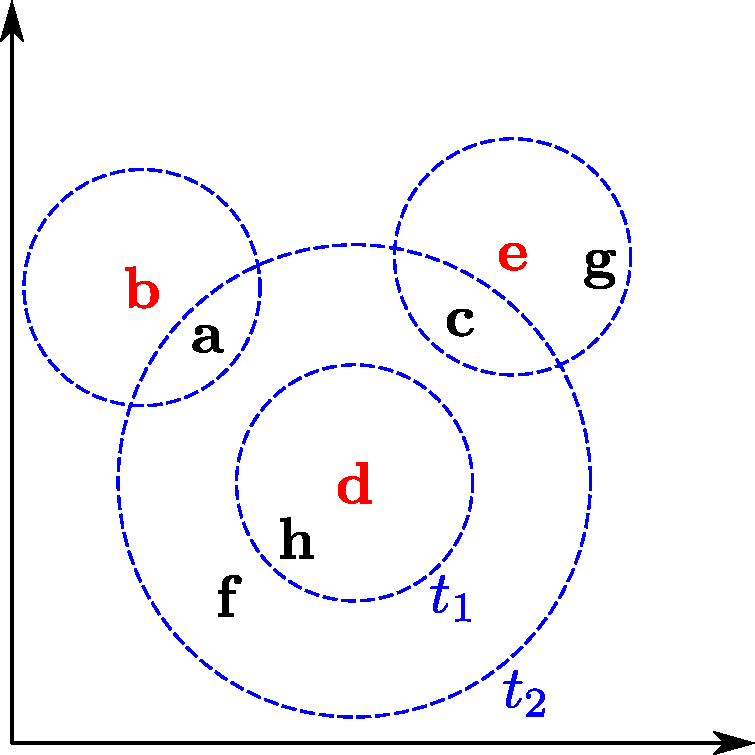
\includegraphics[width=\textwidth]{Graphics/Compactness.pdf}
    \end{subfigure}
    \hfill
    \begin{subfigure}[b]{0.475\textwidth}
        \caption[Connectedness]{\textbf{Connectedness}}
        \label{subfig:Connectedness}            
        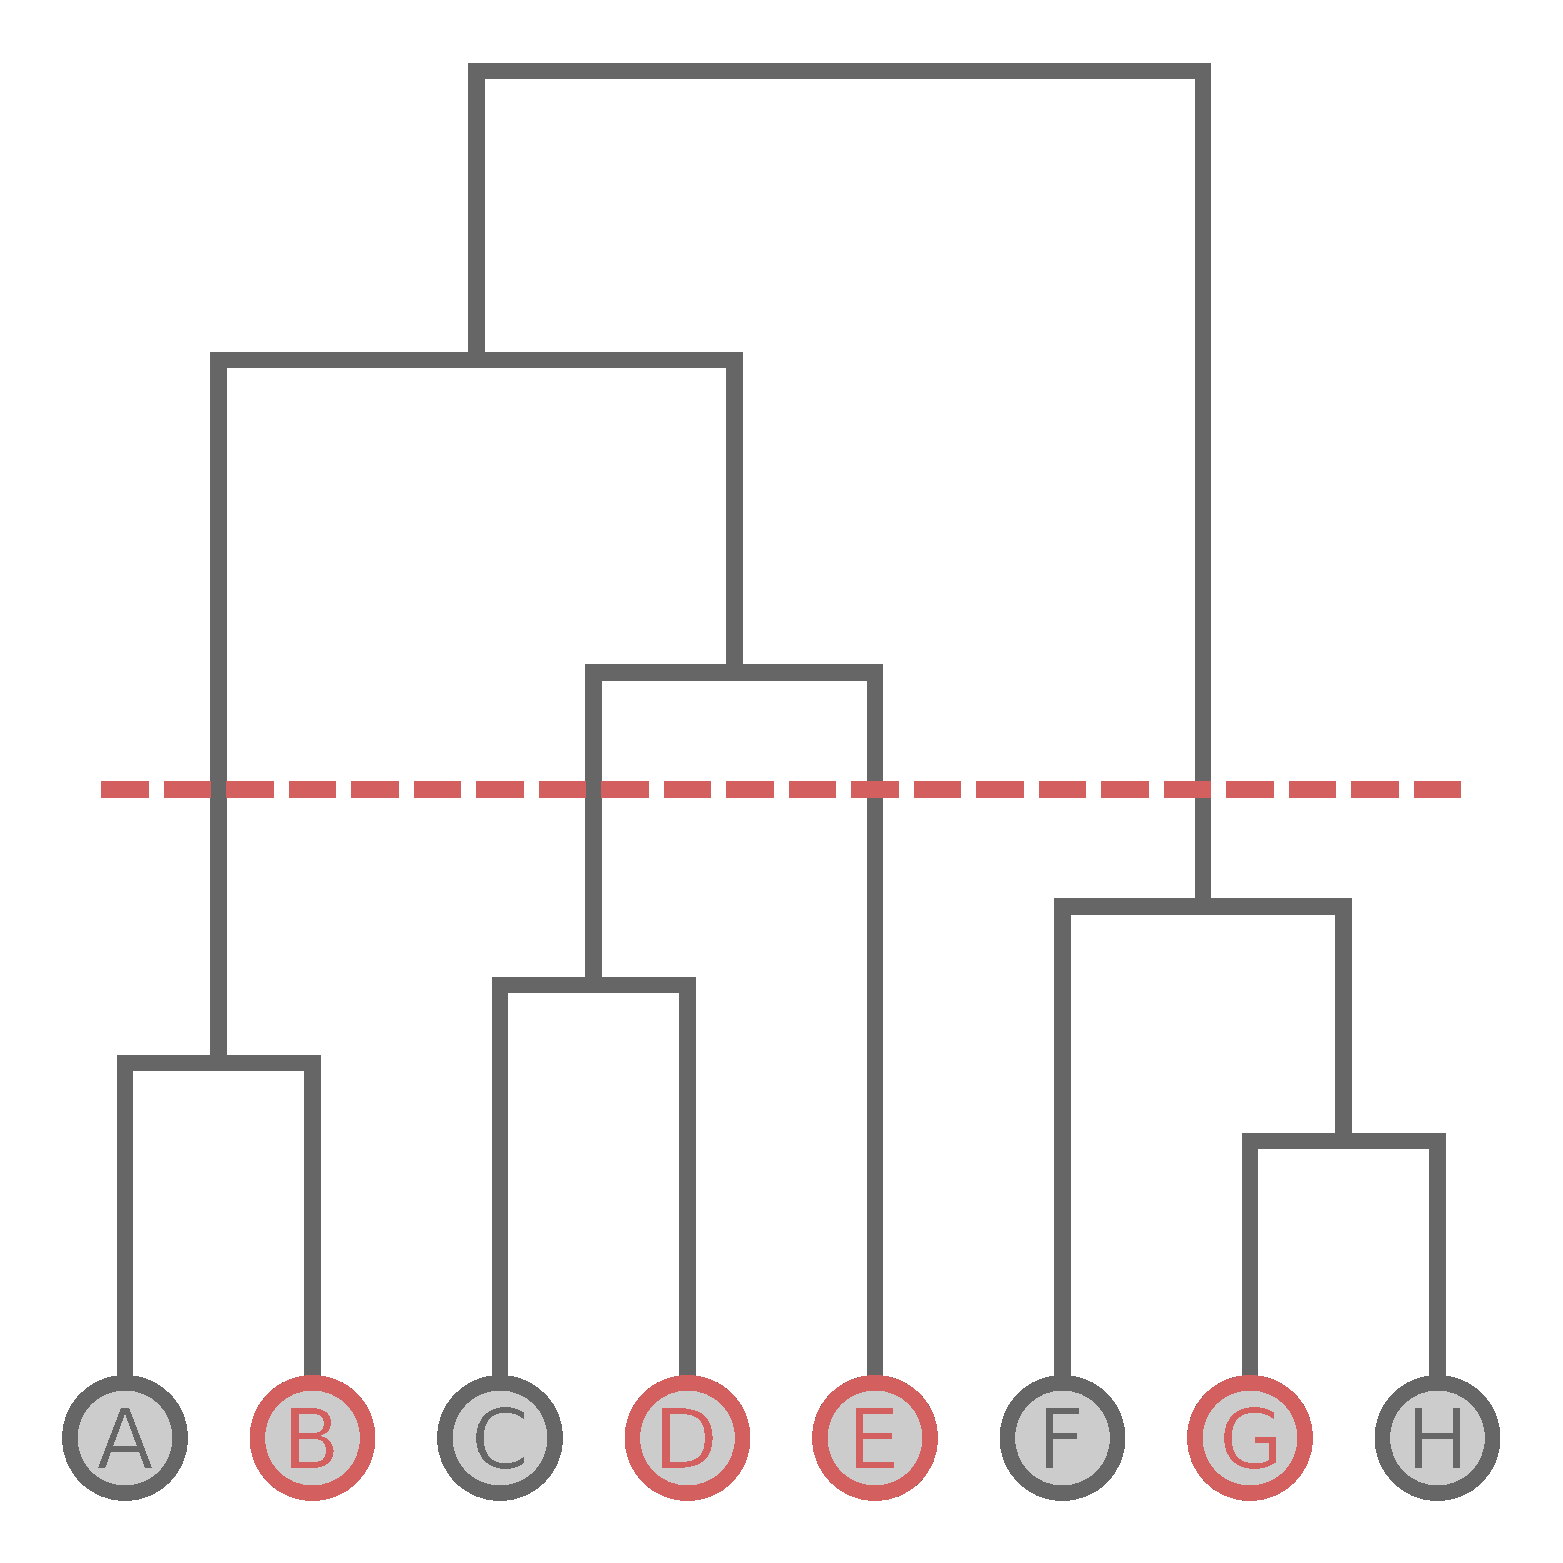
\includegraphics[width=\textwidth]{Graphics/Connectedness.pdf}
    \end{subfigure}
    %\end{adjustbox}
    \caption[Clustering methods]{\textbf{Clustering methods.} .}
    \label{fig:Methods}
\end{figure}

\section{The proposed project}

The present subtype classification of \gls{IAV} is solely based on immunological research on the surface proteins. Since release of this classification around 40 years, with enormous progress in computer technology, have passed. Aside from the raw number of new sequenced genomes of \gls{IAV} in these years, also ways for faster sequence comparisons methods using profiles like k-mer comparisons and more accurate clustering algorithms were paved. Using knowledge from this elapsed time, the classification described in \textcite{noauthor_revision_1980}, will be reevaluated from the perspective of bioinformatics, to possibly find subtle differences to renew the classification with more detailed subgroups. Due to the usage of the raw amount of all high quality sequences available for \gls{IAV}, the clustering into groups were performed without any alignments, searching for a faster, more scaleable and hopefully more accurate method. Instead of alignments a distance measurement using vector representation based on genomic k-mers will be used in combination with high dimensional clustering methods. K-mer distance for genomic comparison was also described in \textcite{edgar_muscle_2004}. To handle the high dimensionality of the used k-mer representation vectors, different dimension reduction methods were described and compared. For clustering hybrid \texttt{HDBSCAN} will be used combining compactness and connectedness for the best accuracy possible aiming for high quality clustering of the huge amount of highly variable \gls{IAV} sequences. Threshold definition is a complex procedure with high impact on the results and will be solved by different approaches involving the Kneedle Algorithm implementing the elbow method for the most appropriate results. This project aims for a clustering based classification of all eight segments of \gls{IAV}, hopefully paving the way for future research to discover more detailed consensus structures and new insights into the molecular life-cycle of the \gls{IAV}. The current subtype classification will support the clustering of segment 4 \gls{HA} in this project and, thereby, create a blueprint to cluster the other segments in a similar way. Nevertheless, due to the lower evolutionary pressure less clusters for the segments not coding for surface proteins are to be expected. For a simple usable new classification, less than 100 clusters per segment would be comfortable and are anticipated, when considering the number of reassortment events in H1N1 proposed in \textcite{nelson_multiple_2008}. 

%\section{WHO classification of \textit{Influenza A Virus}}

%The present day classification of \gls{IAV} is based on the serotype of the virus 

%hybrid clustering combianing both concepts!!

%develop no einteilung sinnvoll fpr secondarys 

%centroid sequences

%To test whether a subset of sequences prefers the tetraloop structure, sequences were clustered using the Unweighted Pair Group Method with Arithmetic Mean (UPGMA)

%To increase the overall efficiency, strategies of next-generation vaccines focus on less variable structures of \gls{HA} and other \gls{IAV} proteins, namely \gls{NA}, \gls{M2} and the \glspl{NP} \autocite{wei_next-generation_2020}. Predicting the overall structure of the \gls{IAV} segments, that are crucial for the virus survival are, thus, essential for drug and vaccine creation against \gls{IAV} and still 

%expected are so und so viele based on the evol variation in dem nature paper wo es nur um H1 ging blabla 1-10 cluster pro subtype

% hierarchical clustering \autocite{gower_minimum_1969}. 

% \blindtext

% \blindtext

% \begin{figure}
%     \centering
%     %\begin{adjustbox}{minipage=\dimexpr\textwidth-2\fboxsep-2\fboxrule,fbox}
%     \begin{subfigure}[b]{0.475\textwidth}
%         \caption[Euclidean]{\textbf{Euclidean}}
%         \label{subfig:Euclidean}
%         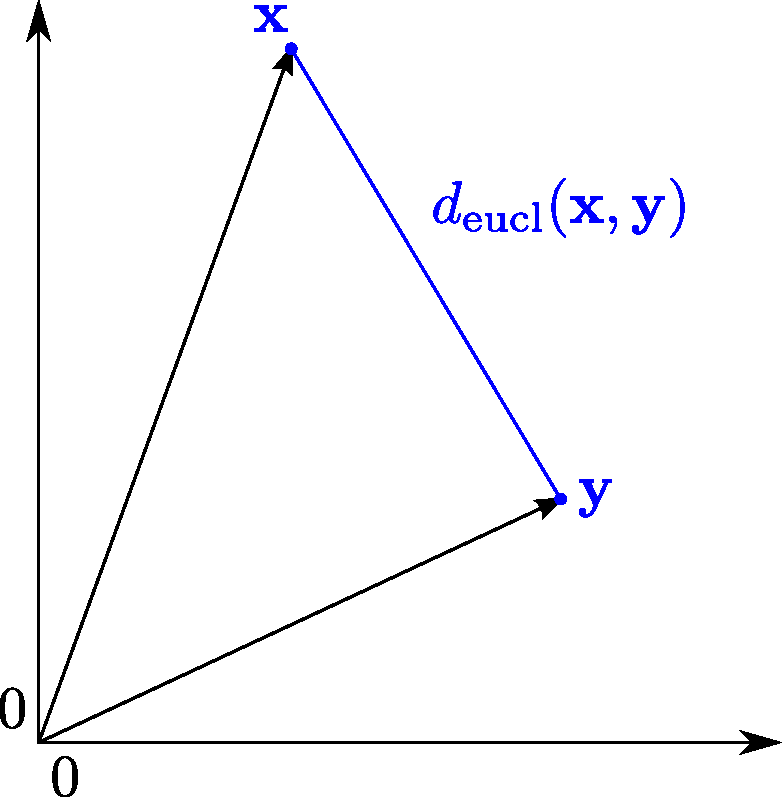
\includegraphics[width=\textwidth]{Graphics/Euclidean.pdf}
%     \end{subfigure}
%     \hfill
%     \begin{subfigure}[b]{0.475\textwidth}
%         \caption[Cosine]{\textbf{Cosine}}
%         \label{subfig:Cosinus}            
%         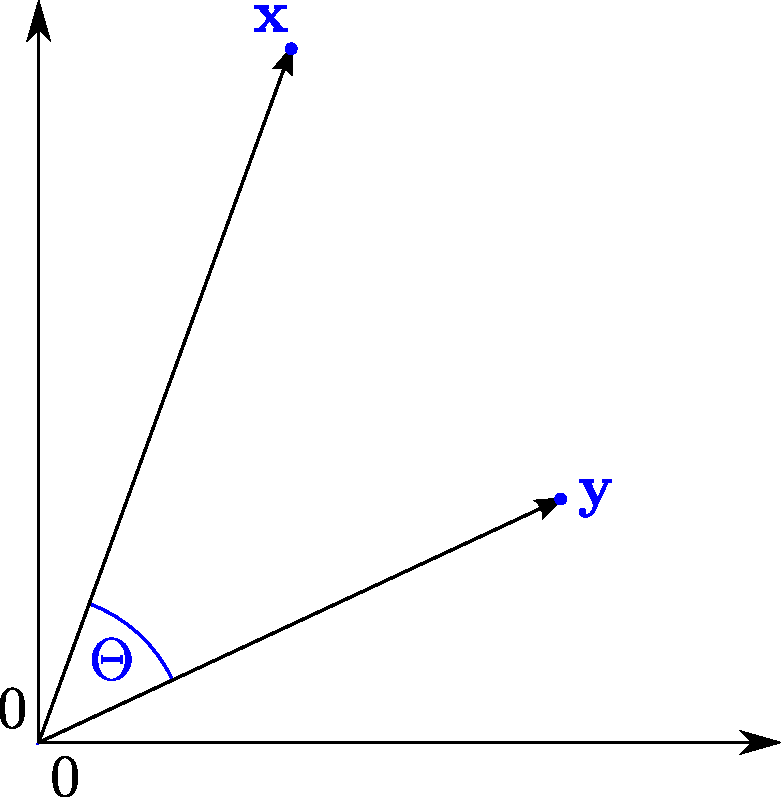
\includegraphics[width=\textwidth]{Graphics/Cosinus.pdf}
%     \end{subfigure}
%     %\end{adjustbox}
%     \caption[Distance Measuring Methods]{\textbf{Distance Measuring Methods.} .}
%     \label{fig:Distance}
% \end{figure}

% \blindtext

% % \begin{fequation}[!hbt]
% %     \begin{empheq}[box=\fbox]{alignat* = -1}
% %         &xL &&&&+zL &&\longrightarrow xL &&&&+zH\\
% %         &xM &&+yL &&+zH &&\longrightarrow xM &&+yL &&+zL\\
% %         &xM &&+yM &&+zL &&\longrightarrow xM &&+yM &&+zH\\
% %         &xH &&+yL &&+zH &&\longrightarrow xH &&+yL &&+zL\\
% %         &xH &&+yM &&+zH &&\longrightarrow xH &&+yM &&+zL\\
% %         & &&\hphantom{++}yH &&+zL &&\longrightarrow &&\hphantom{++}yH &&+zH
% %     \end{empheq}
% %     \caption[]{\textbf{.}}
% %     \label{gl:8.2}
% % \end{fequation}

% \textbf{Normalization with max-norm:} 
% %is the normalization so that the l2 norm of a vector is 1 !!!!!

% \begin{empheq}{alignat = -1}
%     \hat{\mathbf{x}} &= \frac{\mathbf{x}}{\Vert\mathbf{x}\Vert_{\text{max}}}
% \end{empheq}

% \begin{empheq}{alignat = -1}
%     \Vert\hat{\mathbf{x}}\Vert_{\text{max}} &= 1
% \end{empheq}

% \textbf{Cosinus similarity:}

% \begin{empheq}{alignat = -1}
%     %&\cos\angle(\mathbf{x}, \mathbf{y}) &&= \frac{\mathbf{x}^\top\mathbf{y}}{\Vert\mathbf{x}\Vert \cdot \Vert\mathbf{y}\Vert}
%     &\cos(\Theta) &&= \frac{\mathbf{x}^\top\mathbf{y}}{\Vert\mathbf{x}\Vert \cdot \Vert\mathbf{y}\Vert}
% \end{empheq}

% \textbf{cosinus distance}

% \begin{empheq}{alignat = -1}
%     %&d(\mathbf{x},\mathbf{y}) &&= 1 - \cos\angle(\mathbf{x}, \mathbf{y})
%     &d(\mathbf{x},\mathbf{y}) &&= 1 - \cos(\Theta)
% \end{empheq}

% \textbf{euclidean distance:}

% \begin{empheq}{alignat = -1}
%     &d(\mathbf{x},\mathbf{y}) &&= \Vert\mathbf{x} - \mathbf{y}\Vert_2
% \end{empheq}

% %gute anzahl cluster mit nennen 50-100 suoer bzw <100
% %außerdem erwartet, dass ansatzweise wie subtype bei H und N